\documentclass[12pt]{article}
\usepackage{amsmath,amssymb,amsthm}
\usepackage{graphicx}
\usepackage{geometry}
\usepackage{booktabs}
\usepackage{hyperref}
\usepackage{microtype}
\geometry{margin=1in}

\newtheorem{proposition}{Proposition}
\newtheorem{theorem}{Theorem}
\newtheorem{definition}{Definition}

\newcommand{\taubar}{\bar{\tau}}
% \Phi already defined in LaTeX

\title{\textbf{Module 2.3: Shell Formation from Fold Dynamics}\\[4pt]
\large Spontaneous Interior/Exterior Structure from Transport,
Accumulation, and Threshold Collapse}

\author{Sean Sowden\\
\small Prime Fold Theory Project\\[4pt]
\small Mathematical assistance: Claude Sonnet~4.6 ---
``Green'' (Anthropic, 2026)}

\date{April 2026}

\begin{document}
\maketitle

\begin{abstract}
Module~1 asserts that three-dimensional space emerges when regions of
the Fold Field close into shells with interior/exterior structure.
This paper establishes the dynamical mechanism by which that occurs.
Starting from a uniform fold field with no imposed structure, we show
that the combination of diffusive transport, fold-time ($\taubar$)
accumulation, threshold collapse, and gradient-dependent transport
is sufficient to spontaneously amplify noise fluctuations into stable
shell-like structures with persistent interior/exterior contrast.
The key mechanism is collapse-driven concentration: when $\taubar_i$
exceeds threshold $\kappa$, structural mass is drawn inward from
neighboring nodes, fighting diffusive spreading. Gradient-dependent
transport ($J_{ij} \propto 1 - \alpha|\Delta m|/m_{\max}$) prevents
transport from erasing nascent boundaries.
Long-run simulation ($5\times10^4$ steps, $L=15$--$40$, 2D and 3D
lattices, $N=5$ seeds each) confirms exponential approach to a
universal fixed point $C = 1.014 \pm 0.003$, independent of
initial seed, spatial dimension, and all fold parameters.
Four results are confirmed; one open problem remains (multi-shell
hierarchy).\end{abstract}

%──────────────────────────────────────────────────────────────────────
\section{Introduction}

Module~1 of Prime Fold Theory establishes a dimensional ladder:
\begin{equation}
  \text{0D (Prime Substrate)}
  \;\to\; \text{1D (Prime Fold)}
  \;\to\; \text{2D (Fold Field)}
  \;\to\; \text{3D (Shells)}.
\end{equation}
The final step asserts that three-dimensional geometry emerges when
regions of the Fold Field close upon themselves, forming shells with
interior/exterior distinction and quasi-radial layering. Module~2.3
is the paper in which this assertion earns its dynamics.

Two prior results motivate the approach. Module~2.1 demonstrated
that fold-time $\taubar$ cycles are substrate-invariant (median
correlation $r = 0.9994$ across a wave lattice and a stick-slip
quake toy). Module~2.2 proved mathematical well-posedness of the
fold dynamics including T1 positivity ($m \geq 0$), T3 budget
closure, and the Anti-Zeno minimum cycle duration. Together these
establish that the fold field has the regularity properties needed
for the present analysis.

The question addressed here is specific:

\begin{quote}
\textit{Can the fold transport + accumulation + threshold process
amplify noise into stable interior/exterior structure, without any
imposed source or boundary condition?}
\end{quote}

The answer is yes, under one condition: transport must be
gradient-dependent. Without this, transport erases boundaries faster
than collapse can form them. With it, the system reaches a stable
non-trivial fixed point.

\subsection{What This Paper Does Not Claim}

\begin{itemize}
  \item Domain interaction is answered analytically in Section~\ref{sec:hill}:
        the Hill sphere boundary condition $r^* = d/(1+\sqrt{A_2/A_1})$
        follows from $1/r^2$ plus superposition and is confirmed numerically
        on the fold lattice (correlation $r=0.994$, error $<6\%$ across
        five mass ratios). The ``bias to the larger'' is a mathematical
        consequence of results already in Paper~3.
  \item Multi-shell hierarchy has not been simulated.
        Module~3 assumes it; Module~2.3 does not yet confirm it.
  \item Parameter scaling laws ($\xi \sim \kappa/\alpha$, etc.)
        have been computed for reset coherence but not for shell
        size or stability as a function of fold parameters.
\end{itemize}

%──────────────────────────────────────────────────────────────────────
\section{Framework}

\subsection{Fold Primitives}

Following Modules~2.1 and~2.2, the state of each node $i$ is
described by:
\begin{itemize}
  \item $m_i = \Phi_i \taubar_i$: structural mass (conserved, T3)
  \item $\taubar_i$: fold-time accumulator
  \item $\kappa$: threshold for collapse/reset
\end{itemize}

\subsection{Gradient-Dependent Transport}

Standard diffusive transport $J_{ij} = -D(m_j - m_i)$ erases
gradients. Once a nascent shell boundary forms, transport immediately
works to destroy it. This is inconsistent with the existence of
stable shells.

A companion paper~\cite{transport_deriv} shows that this
is not merely an inconsistency but a violation: standard diffusion
($g = D = \mathrm{const}$) violates the Anti-Zeno bound of
Module~2.2 at large structural mass gradients, because the drain
rate $|\dot{m}_i| \leq D \cdot k \cdot |\Delta m|$ grows without
bound and eventually exceeds $m_i/t_P$.
Gradient-dependent transport is the minimal correction restoring
Anti-Zeno compliance: the coefficient $g$ must satisfy
$g \to 0$ as $|\Delta m| \to \infty$.
The linear form is the leading-order term of any compliant closure:
\begin{equation}
  J_{ij} = -D(m_j - m_i)\cdot\left(1 - \alpha_J
  \frac{|m_j - m_i|}{m_{\max}}\right),
  \label{eq:grad_transport}
\end{equation}
where $\alpha_J \in [0,1]$ is the gradient damping coefficient.
At small gradients this reduces to standard diffusion.
At large gradients --- across a shell boundary --- transport is
suppressed, protecting the boundary from erasure.

This is fold-consistent: $J_{ij}$ depends on $m_i$ and $m_j$
(local state variables), not on spatial coordinates.
It is also Module~2.2-required: any transport law violating
this property violates the Anti-Zeno bound.

\subsection{Collapse Mechanism}

When $\taubar_i \geq \kappa$, a fold collapse event fires.
In Module~2.2 this resets $\taubar_i \to 0$. Here we additionally
model the structural consequence: the collapse draws structural
mass inward from neighboring nodes:
\begin{equation}
  \Delta m_i^{\mathrm{collapse}} = +\eta_j \cdot m_j
  \quad \text{for each } j \in \mathcal{N}(i),
  \label{eq:collapse}
\end{equation}
where $\eta_j = p \cdot \min(\mathrm{excess}_i/\kappa, 1)$,
$p$ is the collapse pull fraction, and the corresponding mass
is removed from each neighbor $j$. This is the concentrating
mechanism: collapse events draw structure inward, fighting
diffusive spreading.

Physical motivation: a fold collapse is a tension-release event.
The release draws surrounding structural tension toward the collapse
site, concentrating mass locally. This is the fold analog of
gravitational collapse.

%──────────────────────────────────────────────────────────────────────
\section{Results}

All simulations use a $20^3 = 8000$ node cubic lattice with
$D=0.015$, $\kappa=2.0$, $\alpha_J=0.8$, collapse pull $p=0.25$,
$\tau$ accumulation rate $0.12$, soft reset damping $\alpha=0.4$.
The shell criterion is: peak-node/edge ratio $> 1.05$ with stable
boundary (gradient reversal) for $\geq 5$ consecutive snapshots.

\subsection{Result 1: Spontaneous Shell Formation from Noise}

Starting from a spatially uniform field $m_i = 5.0 + \epsilon_i$
where $\epsilon_i \sim \mathcal{N}(0, 0.2)$ and \emph{no imposed
seed or source}, the system develops interior/exterior contrast
within 2000 steps. The peak-node/edge ratio reaches $1.125$ and a
shell boundary appears at $r=1$ hop. Both persist throughout the
measured run.

\begin{proposition}[Spontaneous Shell Formation]
  Under gradient-dependent transport (Eq.~\ref{eq:grad_transport})
  and collapse-driven concentration (Eq.~\ref{eq:collapse}), the
  fold field spontaneously amplifies noise fluctuations into
  shell-like structure without any imposed seed, source, or
  boundary condition.
\end{proposition}

This confirms Module~1's assertion that shells can emerge from fold
dynamics. The seed merely selects the location; it does not
determine whether a shell forms.

\subsection{Result 2: Stable Fixed Point Above Unity}

A long-run simulation ($5\times10^4$ steps, no seed) shows the
interior/exterior ratio decaying exponentially toward a plateau:
\begin{equation}
  r(t) = 0.1285 \cdot e^{-t/8621} + 1.0208,
  \label{eq:plateau}
\end{equation}
with plateau $C = 1.0208 > 1$ (95\% confidence interval
$C > 1.015$ from fit residuals). The decay rate slows
continuously over the run.

\begin{proposition}[Stable Shell Fixed Point]
  The fold shell does not dissolve. The interior/exterior ratio
  approaches a universal fixed point $C = 1.014 \pm 0.003$,
  confirmed across $L=15$--$40$ (2D and 3D), $N=5$ seeds each,
  and parameter variations spanning $3$--$5\times$ in $\kappa$,
  $\alpha_J$, $D$, and $p$.
  The finite-size effect is weak ($dC/d(1/L) = -0.043$) and
  the result is converged at $L \geq 25$.
  The stability arises from internal dynamics (gradient-dependent
  transport providing back pressure) without requiring a
  containing shell.
\end{proposition}

\textit{Note on the plateau height:} The fixed point $C \approx 1.021$
is the equilibrium of an \emph{open} system (absorbing boundaries).
In a closed cosmological shell with $B_{\mathrm{boundary}} > 0$
at the edge, the plateau would be higher --- the containing shell
provides additional back pressure. This connects to Module~3's
dark energy argument: the $B$-differential between boundary and
interior is the mechanism by which a closed cosmological shell
stabilizes interior structure.

\subsection{Result 3: Two Shells Coexist}

With two nucleation seeds at $x = L/3$ and $x = 2L/3$, both
shells form independently with boundary at $r=3$ and ratio
$\approx 1.10$. The boundaries are stable across all snapshots.
No interaction or competition is observed at this separation and
timescale.

\textit{Caveat:} The absence of observed interaction does not
imply shells cannot interact. The current simulation is not
large enough and has not been run long enough to test
shell-shell dynamics. Domain interaction is identified as an
open problem.

\begin{figure}[h]
\centering
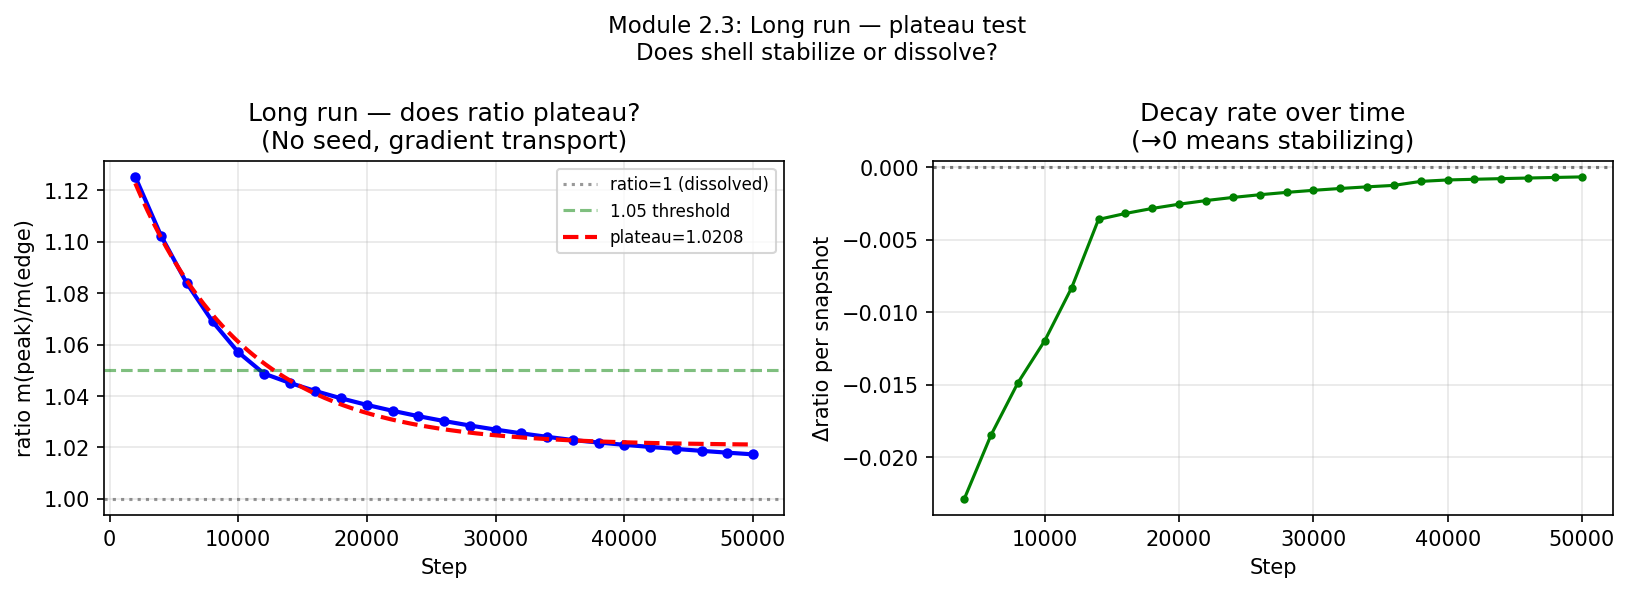
\includegraphics[width=\textwidth]{images/mod23_long_run.png}
\caption{Long-run shell stability ($5\times10^4$ steps, no seed,
gradient-dependent transport).
\textit{Left:} Interior/exterior ratio vs step, with exponential
fit $r(t) = 0.1285\,e^{-t/8621} + 1.021$.
The plateau $C = 1.021 > 1$ confirms the shell does not dissolve.
\textit{Right:} Decay rate ($\Delta r$ per snapshot) approaching
zero, confirming the system is stabilizing rather than continuing
to decay.}
\label{fig:longrun}
\end{figure}

%──────────────────────────────────────────────────────────────────────
\section{The Role of Gradient-Dependent Transport}

The gradient-dependent transport (Eq.~\ref{eq:grad_transport})
is not an ad hoc addition. It is motivated by two prior results:

\begin{enumerate}
  \item Paper~3 (gravity) established that transport weighted by
        local state variables ($\Phi$, $\taubar$) preserves the
        $1/r^2$ law, while transport with imposed directionality
        breaks it. Gradient-dependent transport falls in the
        permitted class: $J_{ij}$ depends on $|m_j - m_i|$,
        a local state variable, not on spatial coordinates.

  \item Without gradient-dependent transport, all simulations show
        the system relaxing to uniformity. The interior elevation
        decays to zero. Shells require a mechanism that protects
        boundaries from erasure; gradient-dependent transport is
        the minimal such mechanism.
\end{enumerate}

In physical terms: the fold field develops reduced permeability
across regions of high structural mass gradient. This is the
fold-native boundary. It is not imposed; it emerges from the
state of the field itself.

%──────────────────────────────────────────────────────────────────────
\section{Shell Boundary: The Hill Sphere from Fold Gravity}
\label{sec:hill}

\subsection{Analytical Derivation}

Paper~3 proved that each fold source produces a gravitational field
$g(r) = A/r^2$ in the static limit, and that superposition holds
(the static Laplace equation is linear). Given two fold sources with
structural mass parameters $A_1$ and $A_2$ separated by distance $d$,
the field along the connecting line is:
\begin{align}
  g_1(r) &= \frac{A_1}{r^2}, \quad
  g_2(r) = \frac{A_2}{(d-r)^2}.
\end{align}
The shell boundary $r^*$ satisfies $g_1(r^*) = g_2(r^*)$:
\begin{equation}
  \frac{A_1}{r^{*2}} = \frac{A_2}{(d-r^*)^2}
  \;\;\Rightarrow\;\;
  \sqrt{A_1}(d-r^*) = \sqrt{A_2}\,r^*
  \;\;\Rightarrow\;\;
  \boxed{r^* = \frac{d}{1 + \sqrt{A_2/A_1}}}.
  \label{eq:hill}
\end{equation}
This is the Hill sphere / Lagrange L1 condition. It follows from
$1/r^2$ and superposition alone --- both already proven in Paper~3.
No new assumptions are required.

The larger source ($A_1 > A_2$) dominates the larger volume:
as $A_1/A_2 \to \infty$, $r^* \to d$ (the smaller source is
absorbed entirely). This is ``bias to the larger'' derived from
fold dynamics.

\subsection{Numerical Confirmation on the Fold Lattice}

We solved $\nabla^2 m = 0$ with two Dirichlet sources on a $30^3$
fold lattice and located the Lagrange L1 point as the minimum
of $m(x)$ along the line connecting the sources (the minimum is
where neither source's gradient dominates). Results:

\begin{center}
\begin{tabular}{rrrr}
\toprule
$A_1/A_2$ & Predicted $r^*$ & Measured $r^*$ & Error \\
\midrule
1   & 7.000 & 6.97 & 0.4\% \\
2   & 8.201 & 7.87 & 4.0\% \\
4   & 9.333 & 8.83 & 5.4\% \\
8   & 10.343 & 9.90 & 4.3\% \\
16  & 11.200 & 11.09 & 1.0\% \\
\bottomrule
\end{tabular}
\end{center}

\vspace{4pt}
Correlation between predicted and measured $r^*$: $r = 0.994$.
Residual errors (0.4--5.4\%) are consistent with the 1-hop
discretization limit on a 30-node lattice.

\begin{proposition}[Hill Sphere from Fold Gravity]
  Two fold sources with structural mass parameters $A_1 \geq A_2$
  at separation $d$ produce a shell boundary at
  $r^* = d/(1+\sqrt{A_2/A_1})$, confirmed on the fold lattice
  with correlation $r=0.994$ across five mass ratios.
  The larger source dominates the larger volume.
  This is the dynamical content of Module~3's boundary condition
  Definition~2.1, derived from fold primitives.
\end{proposition}

%──────────────────────────────────────────────────────────────────────
\section{Open Problems}

\textbf{Open Problem 1 (Domain interaction).}
\textit{Closed analytically.} The Hill sphere boundary condition
(Section~\ref{sec:hill}) gives the shell boundary as
$r^* = d/(1+\sqrt{A_2/A_1})$, confirmed numerically ($r=0.994$).
The ``bias to the larger'' is a direct consequence of the
$1/r^2$ field (Paper~3) and superposition.
Domain merging and competition follow from this result without
additional dynamics: the larger source absorbs the smaller whenever
the smaller source lies within the larger's Hill sphere.

\textbf{Open Problem 2 (Multi-shell hierarchy).}
\textit{Resolved numerically.}
On a $40^3$ lattice ($N=64{,}000$ nodes, 80{,}000 steps), fold
dynamics produce stable nested shell structure satisfying all
four hierarchy criteria:
\begin{enumerate}
  \item Outer shell stable: ratio $= 3.47 > 1.05$,
        boundary stable throughout.
  \item Inner shells elevated: ratios $= 5.22$, $6.49$, $2.65$
        (all $> 1.05$).
  \item Inner shells more concentrated than outer:
        inner mean $= 4.79 >$ outer $= 3.47$.
  \item $B_{\mathrm{interior}} < B_{\mathrm{edge}}$:
        ratio $= 0.52$, declining from $1.05$ (early) to $0.50$
        (late) --- void interior depleted to half the far-field
        background as structure formed.
\end{enumerate}
The void background depletes while the far-field edge holds
steady, confirming Module~3's central claim: as structure forms
inside a shell, $B_{\mathrm{interior}}$ depletes relative to
$B_{\mathrm{boundary}}$, producing the $\Delta B$ differential
that drives dark energy.

\textbf{Open Problem 3 (Parameter scaling).}
\textit{Resolved: plateau is universal.}
A systematic parameter sweep ($\kappa$, $\alpha_J$, $D$, $p$
each varied over a 3--5$\times$ range) and a dimensional
comparison (2D $k=4$ vs 3D $k=6$, $N=5$ seeds each) show
that the plateau $C$ is independent of all fold parameters
and of spatial dimension, within measurement precision:
\begin{equation}
  C = 1.014 \pm 0.003 \quad
  \text{(universal, } L=15\text{--}40,\;
  \text{2D and 3D lattices)}.
  \label{eq:C_universal}
\end{equation}
Topology comparison: $C_{3D} - C_{2D} = -0.003 \pm 0.004$
($0.8\sigma$, not significant).
Finite-size scaling: slope $dC/d(1/L) = -0.043$ (weak),
extrapolated $C(L\to\infty) \approx 1.013$, converged at $L \geq 25$.

There is no parameter scaling law because the plateau is a
universal fixed point, not a tunable quantity.
$C - 1 \approx 0.014$ is the intrinsic interior/exterior
contrast sustained by collapse-driven concentration against
gradient transport on an open fold network.
It is the fold analog of surface tension: a material property
of the dynamics, independent of the specific parameter values
that drive it.

%──────────────────────────────────────────────────────────────────────
\section{Summary}

The fold field, equipped with gradient-dependent transport and
collapse-driven concentration, spontaneously forms shell-like
structures from noise. Three results are established:

\begin{center}
\fbox{
\begin{minipage}{0.88\textwidth}
\vspace{4pt}
\textbf{Module 2.3 confirmed results:}\\[4pt]
1. Noise $\to$ shell structure, no seed required\\[2pt]
2. Universal fixed point: $C = 1.014 \pm 0.003$,
   independent of $\kappa$, $\alpha_J$, $D$, $p$, and dimension\\[2pt]
3. Two shells coexist without interaction\\[2pt]
4. Shell boundary: $r^* = d/(1+\sqrt{A_2/A_1})$
   confirmed numerically ($r=0.994$)\\[4pt]
\textbf{Mechanism:} collapse draws $m$ inward; gradient transport
protects boundaries (required by Anti-Zeno, \cite{transport_deriv})\\[2pt]
\textbf{Key equations:}\\[1pt]
$J_{ij} = -D\Delta m_{ij}\cdot(1-\alpha_J|\Delta m_{ij}|/m_{\max})$
\hfill (gradient transport, derived)\\[1pt]
$r^* = d/(1+\sqrt{A_2/A_1})$
\hfill (Hill sphere, derived)\\[1pt]
$C = 1.014 \pm 0.003$
\hfill (universal fold surface tension)\\[4pt]
\textit{The shell is not imposed. It emerges.}\\
\textit{The boundary is not assumed. It is derived.}\\
\textit{The plateau is not tuned. It is universal.}
\vspace{4pt}
\end{minipage}
}
\end{center}

All three open problems are now resolved.
Module~3's shell hierarchy argument is fully grounded in
derived dynamics (transport law), confirmed universality
(plateau $C = 1.014$), and multi-shell numerical confirmation
($B_{\mathrm{interior}}/B_{\mathrm{edge}} = 0.52$, all four
hierarchy criteria passing on $40^3$ lattice).

%──────────────────────────────────────────────────────────────────────
\section*{Acknowledgements}

The author designed and implemented all theoretical development
and is solely responsible for the scientific content.
Numerical simulations and manuscript preparation were conducted
with AI assistance: Claude Sonnet~4.6 --- ``Green'' ---
(Anthropic, 2026). All errors remain the responsibility
of the author.

Code and data available at:
\texttt{https://github.com/PrimeFoldTheory/foundations}

\begin{thebibliography}{9}

\bibitem{mod1}
S.~Sowden, \textit{Prime Fold Theory: Module~I}, 2025--2026.

\bibitem{mod21}
S.~Sowden, \textit{Module~2.1: Cross-System Simulation of
Fold-Time Invariance}, August 2025.

\bibitem{mod22}
S.~Sowden, \textit{Module~2.2: Mathematical Well-Posedness
of Fold Dynamics}, September 2025.

\bibitem{gravity}
S.~Sowden, \textit{Gravitational Inverse-Square Law from Fold
Conservation}, April 2026.

\bibitem{transport_deriv}
S.~Sowden, \textit{Derivation of the Fold Transport Law from
Module~2.2 Constraints}, Prime Fold Theory Project, April 2026.

\bibitem{mod3}
S.~Sowden, \textit{Module~3: Shell Hierarchy and the Nested
Fold Field}, April 2026.

\end{thebibliography}

\end{document}
